\section{Implementacja}
W celu przeprowadzenia prac badawczych na temat konsekwencji zaproponowanych mechanizmów, koniecznym było zaimplementowanie podstawowego kompilatora. 
\subsection{Fazy kompilacji}
\label{Compilation_phases}
Ze względu na nietypową konstrukcję C-=-1, proces kompilacji musi być dłuższy oraz ostrożniej zaprojektowany niż w typowym statycznie typowanym języku programowania.
Ponieważ użytkownik ma pisać kod, który będzie modyfikował wewnętrzne struktury danych kompilatora, musi on wiedzieć kiedy które jej elementy są gotowe.
Kolejność operacji wykonywanych przez kompilator, staje się przez to częścią języka.
\begin{enumerate}
    \item Budowa reprezentacji pośredniej atrybutów
    \item Zebranie definicji funkcji i typów
    \item Przyłączenie atrybutów
    \item Budowa reprezentacji pośredniej funkcji i typów
    \item Wykonanie meta-funkcji atrybutów
    \item Zastąpienie wyrażeń zawierających statyczną refleksję ich wynikami
    \item Zapisanie reprezentacji pośredniej paczki
    \item (opcjonalne) Konwersja do postaci pośredniej LLVM i kompilacja do kodu maszynowego
\end{enumerate}

Współczesne kompilatory są typowo skonstruowane z trzech części: front-end, middle-end i back-end [9].
Zadaniem front-endu jest walidacja składni, weryfikacja typów oraz buduje reprezentację pośrednią kodu. Middle-end, operując na tych strukturach danych dokonuje optymalizacji niezależnych od maszyny docelowej.
Na koniec back-end optymalizuje kod pod kątem konkretnej architektury procesora i generuje kod maszynowy.

Ze względu na nietypowe wymagania C-=-1, zastosowano nowy podział odpowiedzialności.
W przeciwieństwie do typowych języków programowania, implementowany kompilator nie może wygenerować reprezentacji pośredniej programu jako jeden krok.
Punkt 3 procesu kompilacji, może wpływać na wybór rozwiązywanie przeciążeń funkcji.

Kompilator C-=-1 dzieli się na następujące części:
\begin{enumerate}
    \item Frontend
    \item Interpreter
    \item Optimiser
    \item Serialisator
    \item Backend Interface
    \item Backend
\end{enumerate}
Część z tych komponentów nazywa się tak samo jak w klasycznej architekturze. Jest to zabieg celowy, ponieważ pełnią one te same funkcje. Dodatkowe komponenty kompilatora które zostały wydzielone to: Interpreter, Serialisator oraz Backend Interface. Nazwa Optimiser została wybrana ponieważ wyrażenie „middle-end” rzadko występuje w literaturze a wybrany termin jest bardziej deskryptywny.

Ponieważ częścią kontraktu pomiędzy programistą a językiem C-=-1 jest kod wykonywany w czasie kompilacji, jednym z wydzielonych komponentów jest Interpreter. Operuje on na CIR omówionej w rozdziale 3.4. Interpreter stanowi najważniejszy komponent kompilatora, ponieważ większość transformacji odbywa się za jego pomocą. Szczegółowe działanie tego komponentu jest opisane w rozdziale 4.3.

Optimiser został dodany do struktury kompilatora, aby zapewnić możliwość dalszego rozwoju i dla kompletności projektu. Nie został jednak zaimplementowany.

Serializator jest odpowiedzialny za zapisywanie i odczytywanie struktur danych kompilatora z formy tekstowej. Służy to zarządzaniu zależnościami. Zserializowaną w ten sposób paczkę można dystrybuować za pomocą serwisu takiego jak NPM oraz używać w innych projektach. Ponieważ zawartością takiego modułu jest zserializowane, niezależne od platformy CIR, nie istnieje problem binarnej kompatybilności. Kompilacja programu używając paczek C-=-1 jest ekwiwalentna do kompilowania programu C++ używając zależności wyłącznie w formie kodu źródłowego. Cały program jest kompilowany tym samym narzędziem, na tej samej maszynie i z tymi samymi flagami. Serializator jest dokładnie opisany w rozdziale 4.4 a mechanizm zarządzania zależnościami w rozdziale 4.2.1.

Kompilator C-=-1 używa LLVM jako back-endu. W związku z tym, koniecznym jest przetłumaczenie CIR na reprezentację pośrednią LLVM (w dalszej części pracy nazywanej LIR). Dlatego do kompilatora dodano element Backend Interface który dokonuje tej konwersji. Obydwa te komponenty są opisane w rozdziałach 4.6 oraz 4.5.
 
\begin{figure}[]
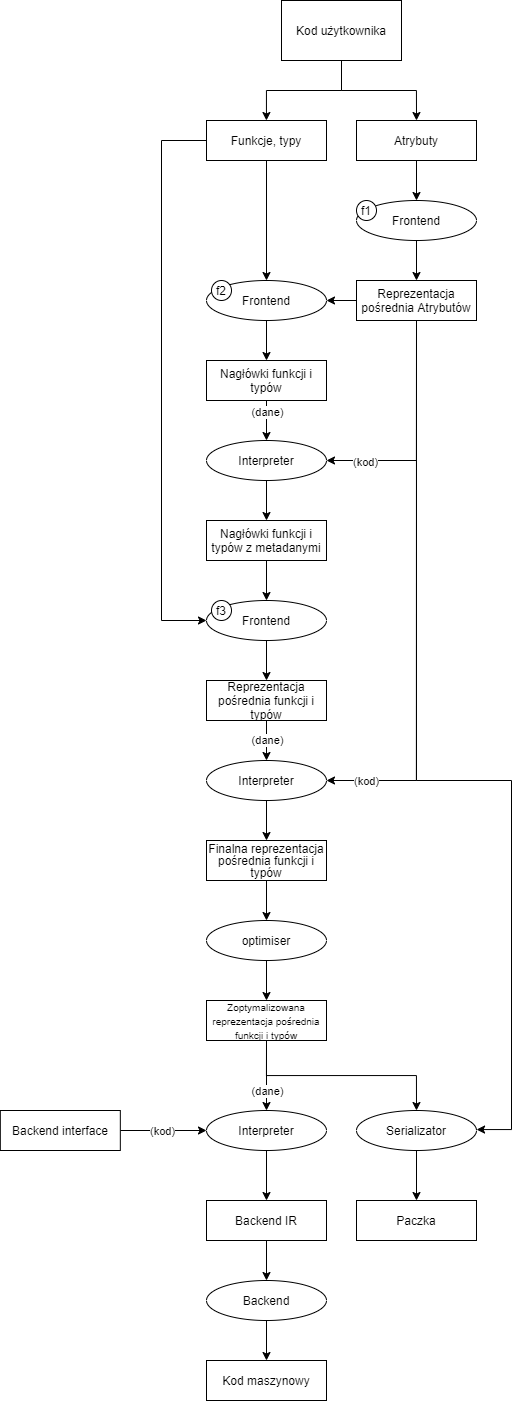
\includegraphics[scale=0.8]{img/compilation_process.png}
\caption{diagram procesu kompilacji języka C-=-1}
\centering
\end{figure}
\subsection{Front-end}
Front-end kompilatora C-=-1 jest odpowiedzialny za interakcje z tekstem kodu źródłowego. Rysunek 1 przedstawia diagram procesu kompilacji. Front-end gra w nim kluczową rolę w początkowych fazach, przetwarzając zawartość plików źródłowych. Sposób w który źródła są odczytywane oraz analizowane jest opisany w rozdziale 4.2.1.
Zrealizowanie tego procesu wymagało aby ten komponent kompilatora potrafił funkcjonować w różnych trybach w zależności od obecnie wykonywanego kroku. Ponadto, ponieważ w C-=-1, w przeciwieństwie do C++, kolejność deklaracji nie ma znaczenia, front-end musiał radzić sobie z zależnościami kołowymi. Ogół działania front-endu jest opisany w rozdziale 4.2.2.
\subsubsection{Parser}
Do parsowania tekstu wejściowego, użyto generatora parserów Rose [10]. Jest to narzędzie bazujące na Antlr, które znacząco ułatwia manipulowanie drzewem składniowym (ang. AST). Te dodatkowe możliwości są wykorzystywane przy przetwarzaniu szablonów (rozdział 4.2.5).
Kompilator trzyma w pamięci tylko jedno drzewo rozkładu na raz, co oznacza że każdy plik jest wczytywany wielokrotnie. Ta decyzja ma ograniczyć ilość zużywanej w danym momencie pamięci operacyjnej.
W celu analizy tekstu wejściowego użyto wizytatorów. Jest to typowy wzorzec projektowy w 
\subsubsection{Fazy przetwarzania plików źródłowych}

\subsubsection{Zarządzanie zależnościami}

\subsubsection{Import symboli zewnętrznych}

\subsubsection{Reprezentacja pośrednia}
Reprezentacja pośrednia jest istotnym elementem języka, na którym opiera się meta-programowanie w C-=-1. W związku z czym, każda jej część jest udokumentowana w załączniku 1. Wewnątrz kompilatora, reprezentacja pośrednia jest przechowywana w ramach struktur danych interpretera (rozdział 4.3.1), aby umożliwić interakcję z interpretowanym kodem.
Ponieważ użytkownik C-=-1 ma operować na CIR (C-=-1 Intermidiate Representation), jej struktura jest bliska językowi który reprezentuje. Poza dodaniem specjalnych typów instrukcji struktura CIR jest niemal identyczna z C-=-1. Takie podejście ma zarówno wady i zalety. 
Z jednej strony sprawia ono, że błędy w kompilatorze są łatwiejsze, oraz front-end jest łatwiejszy do implementacji. Przez podobieństwo do kodu źródłowego sprawia, że różnice względem poprawnego rezultatu są dużo bardziej oczywiste od bardziej abstrakcyjnych reprezentacji.
Taka reprezentacja jest jednak dużo trudniejsza do interpretowania. W przeciwieństwie do języków takich jak CIL (Common Intermediate Language) [11], CIR nie operuje abstrakcyjnej maszynie stosownej. Szczegółowy opis działania interpretera znajduje się w rozdziale 4.3.
Główne różnice w strukturze między C-=-1 a CIR polegają na bardziej dosłownym wyrażeniu programu. W reprezentacji pośredniej wszystkie odniesienia są w pełni kwalifikowane nazwą paczki i przestrzenią nazw. Finalizatory są wywoływane wprost, używając specjalnej instrukcji. Zamiast rozwiązywania przeciążeń funkcji, CIR odnosi się do konkretnego przeciążenia przez unikatowy identyfikator.
\subsubsection{Szablony}

\subsection{Interpreter}
Interpreter C-=-1 operuje na reprezentacji pośredniej tego języka (rozdział 4.2.5).
\subsubsection{Reprezentacja obiektów}
\subsubsection{Wykonanie kodu}
\subsubsection{Funkcje specjalne}
\subsubsection{Referencje do obiektów C++}
\subsection{Serializator}
\subsection{Backend Interface}
Odpowiedzialnością interfejsu back-endu jest przetłumaczenie CIR na LIR. Na tym etapie kompilacji, cała reprezentacja pośrednia C-=-1 jest przechowywana w ramach struktur danych interpretera. Stworzyło to okazję do napisania części kompilatora w języku docelowym.
To rozwiązanie zapewniło bezpieczeństwo typów w tej części kodu oraz ułatwiło rozwój C-=-1. Tworzenie kompilatora w języku docelowym jest typowym w konstrukcji tego typu narzędzi. Program tak skonstruowany nazywają się „Bootstrapping Compiler” [12]. 
Implementacja tej części kompilatora w C-=-1 ułatwiła rozwój tego języka. Jedną z głównych zalet narzędzia skonstruowanego w ten sposób jest istnienie dużego projektu w języku docelowym. Wymusza to szybszy rozwój języka oraz umożliwia znajdowanie błędów w kompilatorze.
\subsubsection{Funkcje eksponowane przez kompilator}
Używając mechanizmów, opisanych w rozdziałach 4.3.3 oraz 4.3.4, interfejsowi backendu narzędzie do budowy LIR zdefiniowane w LLVM. Za jego pomocą może generować reprezentacje pośrednią LLVM.
W ramach biblioteki backendu, istnieje cała gama funkcji oraz typów używanych do emitowania reprezentacji pośredniej. Duża ich część została wyeksponowana interfejsowi backendu.
\subsubsection{Implementacja interfejsu backendu}
Razem z plikiem wykonywalnym kompilatora, dystrybuowany jest kod źródłowy paczki, zawierającej interfejs backendu. Przed kompilacją kodu użytkownika, kompilator wczytuje ten moduł. Zaletą tego rozwiązania jest możliwość wymiany tego komponentu, bez rekompilacji całego narzędzia.
Po załadowaniu tej paczki, kompilator szuka w niej zestawu funkcji createTranslator która służy jako punkt wejścia dla interfejsu. Ma ona za zadanie zainicjować paczkę oraz zwrócić implementacje interfejsu ITranslator. Zostanie ona użyta do generowania LIR dla poszczególnych struktur języka.

\subsection{Backend}
Do generowania kodu maszynowego została wykorzystana biblioteka LLVM.
\subsection{Biblioteka standardowa}

\subsection{Narzędzia dodatkowe}

\subsubsection{Tryb interaktywny}

\subsubsection{Debugger}

\subsubsection{Wtyczka do VS code}
\subsection{Wyzwania}
Generyki są zależne od kontekstu
Specjalne operatory nameof typeof etc
odchudzenie kompilatora przez trzymanie metadanych o funkcjach jako runtime value i funkcje do dostępu do tego jako klucz-wartość